\documentclass[tikz,border=3pt]{standalone}
\usepackage[utf8]{inputenc}
\usepackage[T1]{fontenc}
\usepackage{lmodern}
\renewcommand{\familydefault}{\sfdefault}
\usepackage{sansmath}\sansmath
\usepackage{pgfplots}\pgfplotsset{compat=1.18,/pgf/number format/use comma,/pgf/number format/1000 sep={.}}
\usetikzlibrary{arrows.meta,calc,positioning,decorations.pathmorphing,patterns}
% paleta del sitio
\definecolor{nar}{HTML}{E8680C}\definecolor{narc}{HTML}{FFB35C}\definecolor{hielo}{HTML}{FFF3E8}
\definecolor{tinta}{HTML}{1D1D1F}\definecolor{gris}{HTML}{6E6E73}\definecolor{lila}{HTML}{7C5CF0}
\definecolor{azul}{HTML}{2F6FD6}\definecolor{menta}{HTML}{17A673}\definecolor{coral}{HTML}{E8342A}
\begin{document}
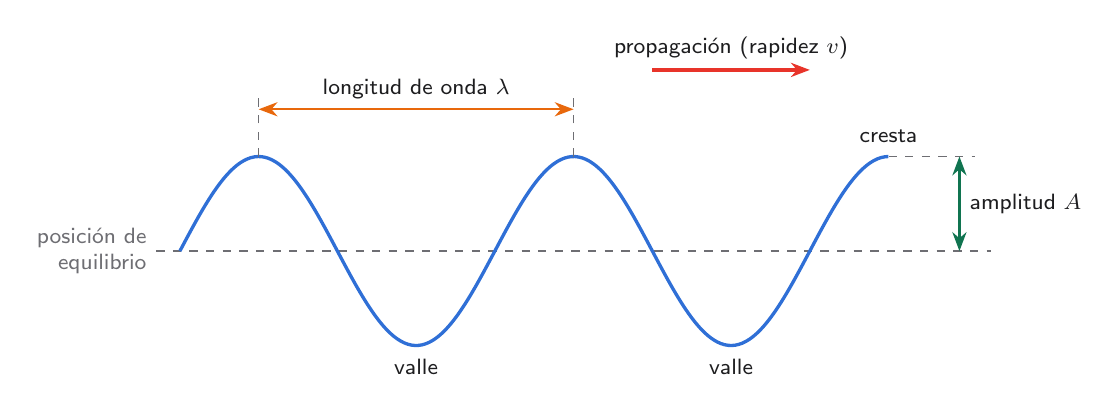
\begin{tikzpicture}[font=\footnotesize,>={Stealth[length=2.4mm]}]
\draw[gris,dashed] (-0.3,0) -- (10.3,0);
\node[gris,left,align=right] at (-0.3,0) {posición de\\equilibrio};
\draw[very thick,azul,domain=0:9,samples=200,smooth] plot (\x,{1.2*sin(90*\x)});
\draw[gris,thin,dashed] (1,1.2) -- (1,2.0) (5,1.2) -- (5,2.0);
\draw[<->,thick,nar] (1,1.8) -- (5,1.8) node[midway,above,text=tinta] {longitud de onda $\lambda$};
\node[above,text=tinta] at (9,1.25) {cresta};
\node[below,text=tinta] at (3,-1.25) {valle};
\node[below,text=tinta] at (7,-1.25) {valle};
\draw[gris,thin,dashed] (9,1.2) -- (10.1,1.2);
\draw[<->,thick,menta!70!black] (9.9,0) -- (9.9,1.2) node[midway,right,text=tinta] {amplitud $A$};
\draw[->,very thick,coral] (6,2.3) -- (8,2.3) node[midway,above,text=tinta] {propagación (rapidez $v$)};
\end{tikzpicture}
\end{document}
